\chapter{User Manual}
The development timelines shown in Figures~\ref{fig:fallQuarter},~\ref{fig:winterQuarter},~and~\ref{fig:springQuarter} below depict a set of tasks that need to be completed throughout the year. We used a Gantt Chart to break down our project into smaller deliverables. The horizontal blue lines split our work into three main sections: development, relationship, and documentation. We separated the larger chart into three individual charts, each corresponding to an individual academic school year.

\begin{figure}[htb]
\centering
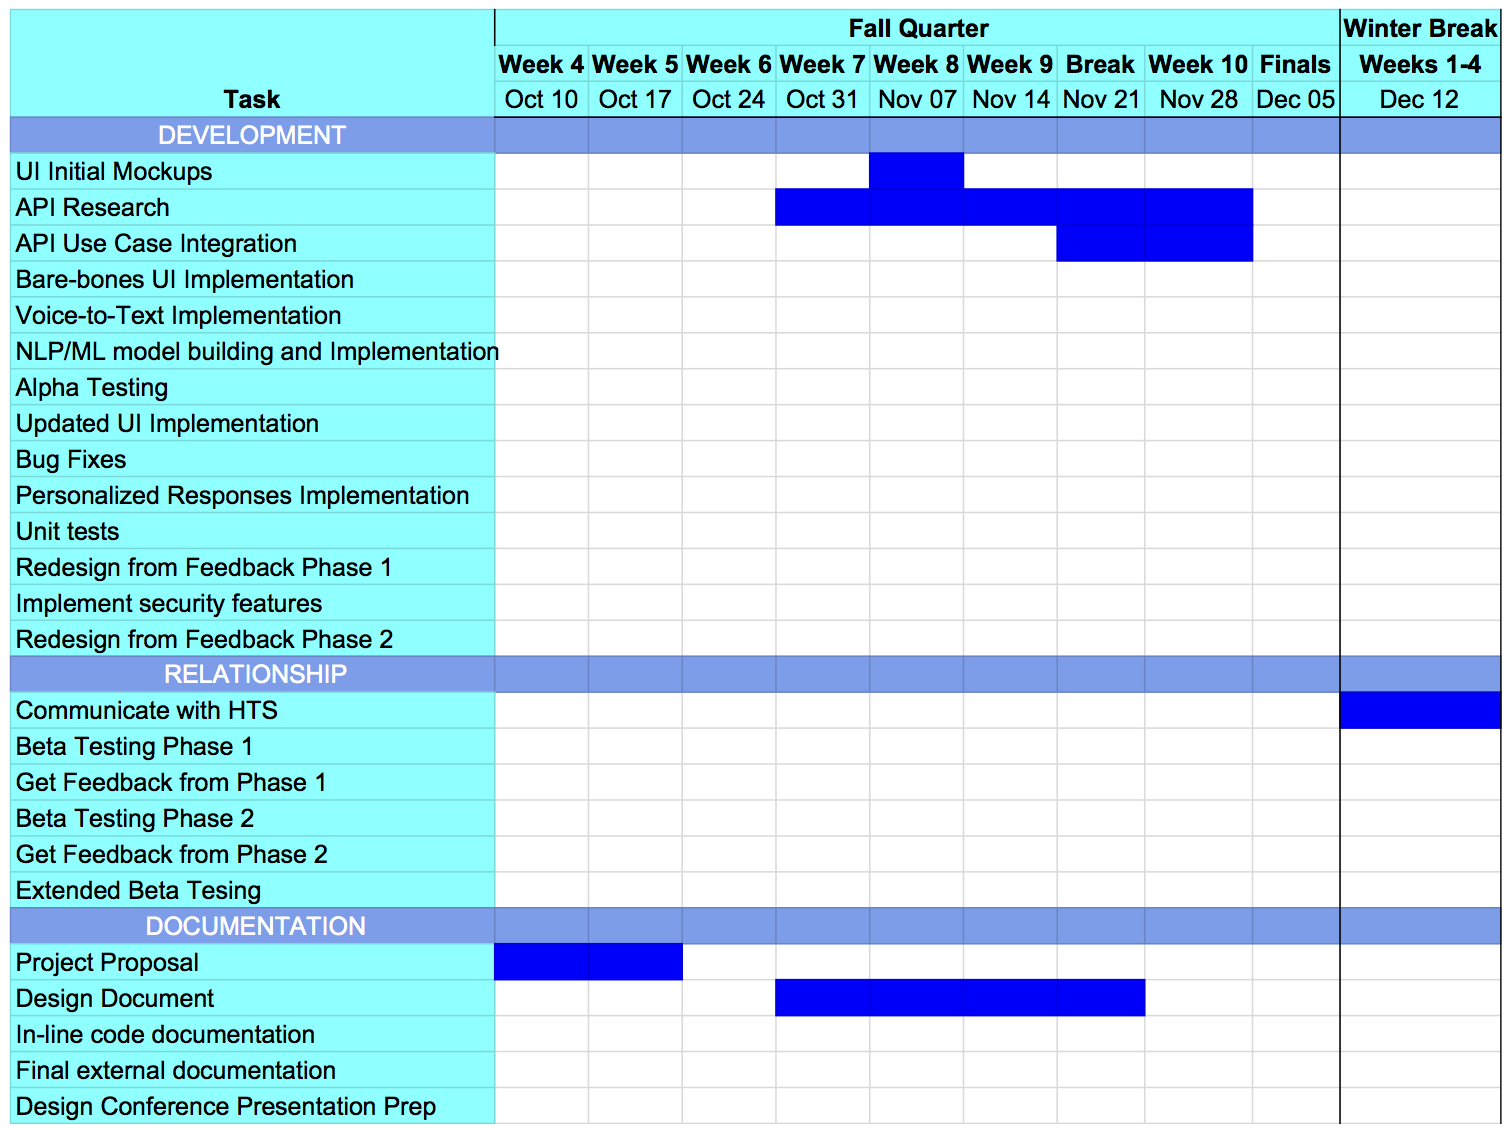
\includegraphics[width =\textwidth]{fallQuarter.png}
\caption{Fall Quarter Development Timeline Gantt Chart}
\label{fig:fallQuarter}
\end{figure}

\begin{figure}[htb]
\centering
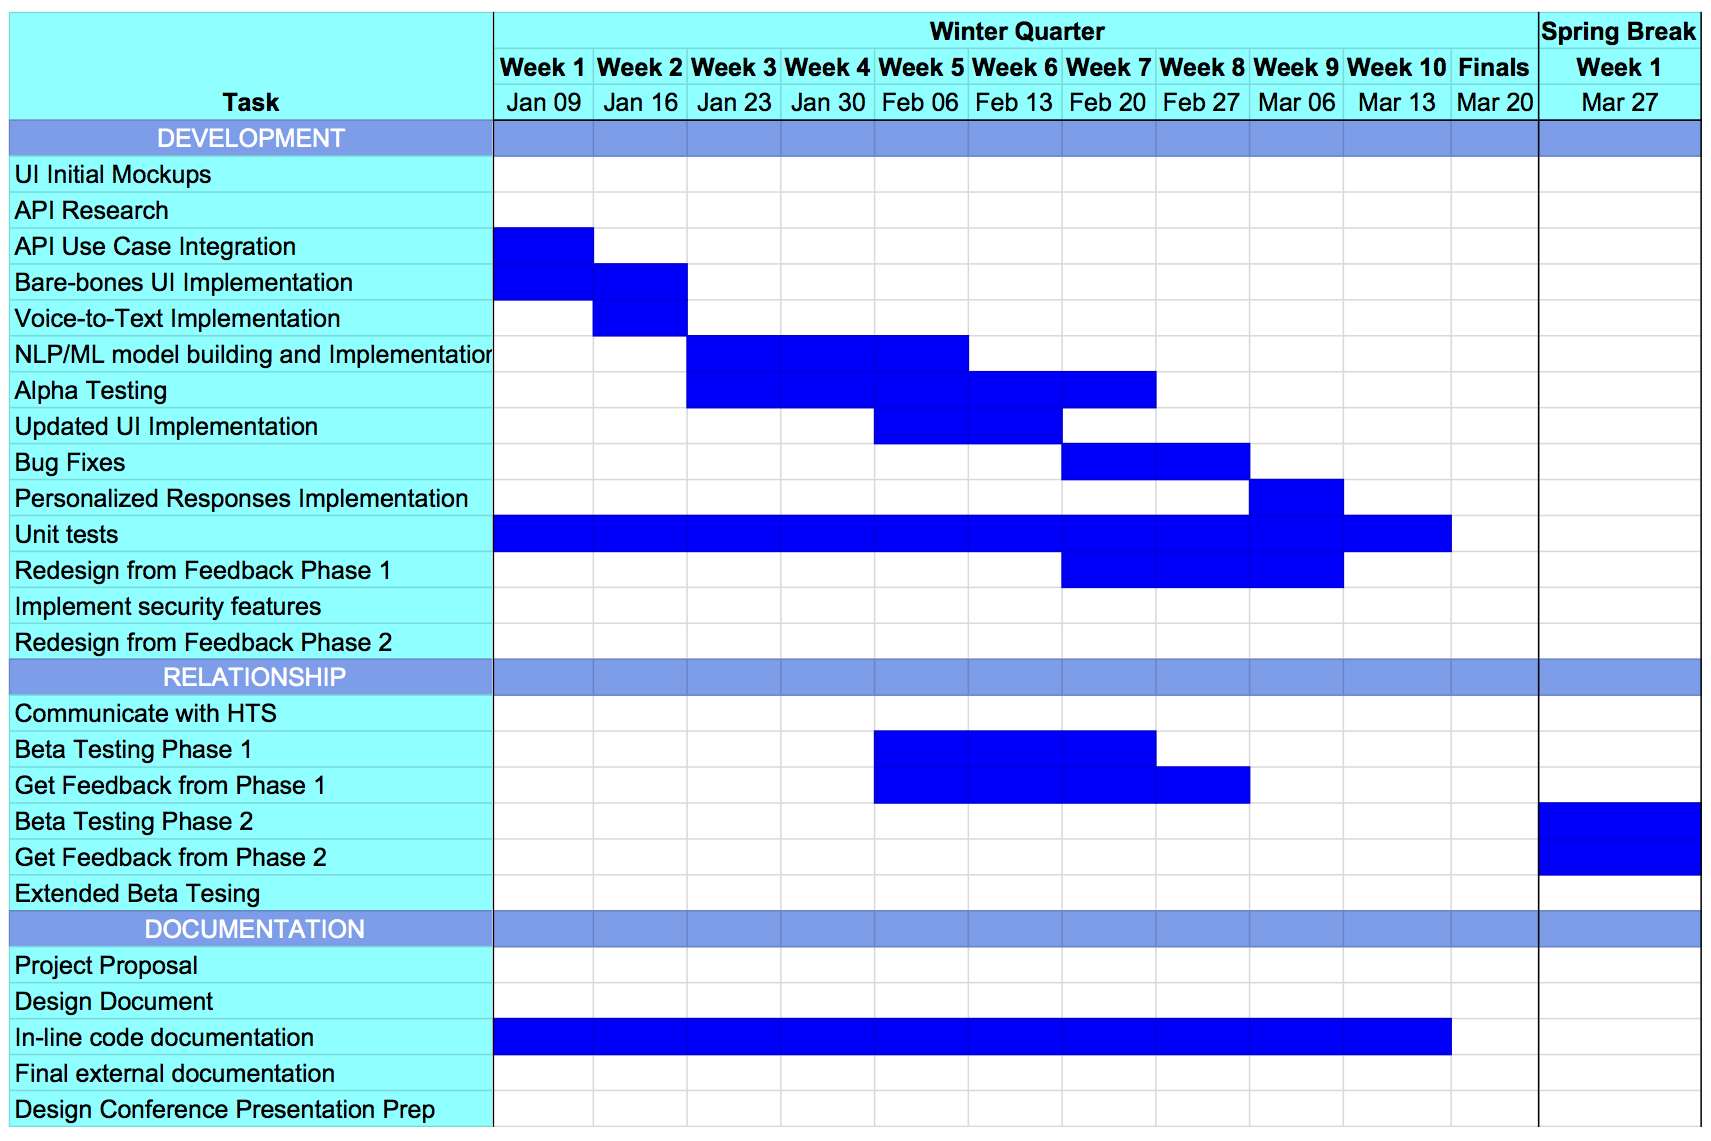
\includegraphics[width =\textwidth]{winterQuarter.png}
\caption{Winter Quarter Development Timeline Gantt Chart}
\label{fig:winterQuarter}
\end{figure}

\begin{figure}[htb]
\centering
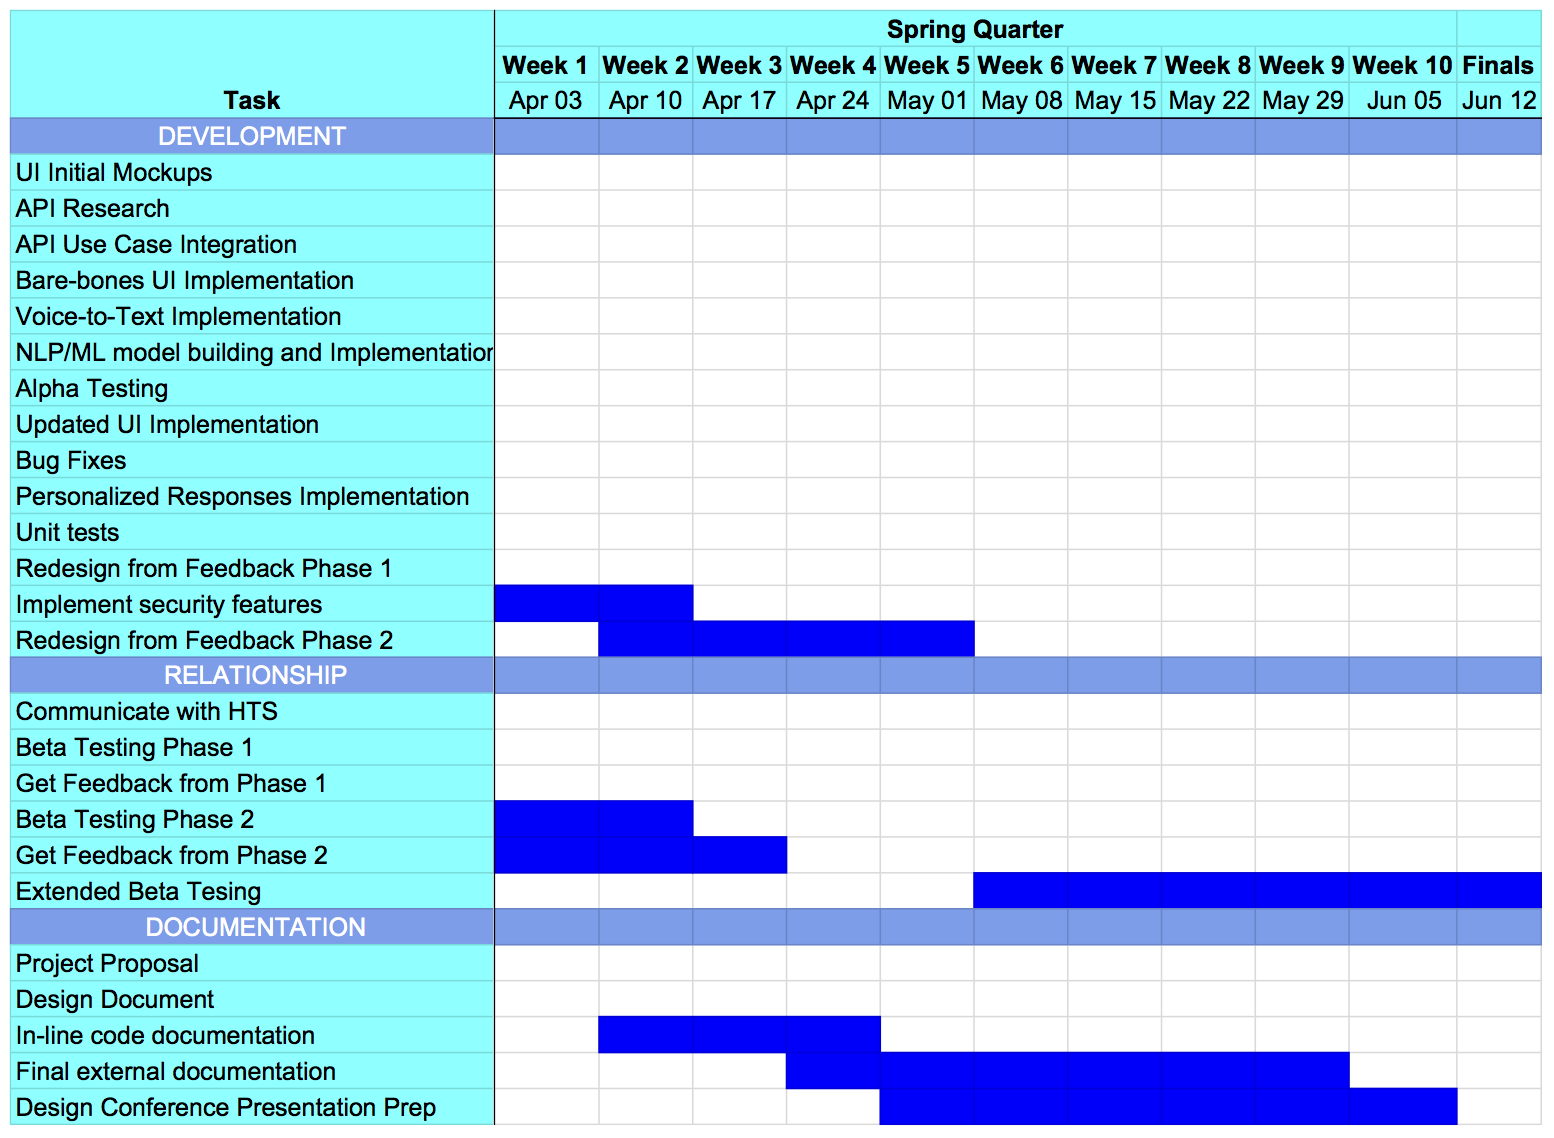
\includegraphics[width =\textwidth]{springQuarter.png}
\caption{Spring Quarter Development Timeline Gantt Chart}
\label{fig:springQuarter}
\end{figure}